\section{Notes (Excluded from Final Paper)}

% \subsection{$\VR(\cp^n)$}

% \cite[Corollary 7.10]{lim2020vietoris} states that there exists some $\alpha_n\in (0,\arccos(-1/3))$ such that $\VR_r(\cp^n)$ is homotopy equivalent to $\cp^n$ for any $r\in (0,\alpha_n)$. 
% This is not enough for us, because we want a `long' enough bar in the usual barcode (assuming the Steenrod barcode is almost trivial). 

% If we consider the rational coefficients, then the rational filling radius of $\cp^n$ being $1/2\arccos(-1/3)$ can be helpful to us. %reference: \url{https://www.sciencedirect.com/science/article/pii/0166864191901223}
% The proposition in \cref{ss:filling_radius} gives the fundamental bar  $(0,\arccos(-1/3))\in \Hbarc[\mathbb{Q}]{m}{\cM}$.

% The next question will be what are the Steenrod barcodes (over $\mathbb{Q}$) of $\cp^n$. This can still be a hard question, because we do not know the homotopy type of $\VR_r(\cp^n)$ for $r$ in the fundamental bar.

%\ling{to-do's for Ling: reorganize Section 5.5. Mention the gaps we have, e.g. what is lacking if we were to apply the same approach ($\VR(S^n/\sim)\simeq \VR(S^n)/\sim$ is not that difficult, but $\VR(S^n)/\sim$ is hard to understand)}

%We estimate the bottleneck distance $\db$ between the Steenrod barcodes of the two space $\VS^n$ and $\rp^n$, and show that it provides a better (lower-bound) approximation of the Gromov--Hausdorff distance than $\db$ between the standard barcodes.
\subsection{}

Let $X$ be an $n$-dimensional manifold.
The \defn{first critical value} of the Vietoris-Rips filtration of a metric space $X$ is some $\alpha\geq 0$ such that 
\begin{itemize}
    \item for any $0 \leq t\leq t'\leq \alpha$, $\VR_t(X)\simeq X$ and $\VR_{t}(X) \hookrightarrow \VR_{t'}(X)$ is a homotopy equivalence;
    \item $\VR_t(X)$ changes homotopy type at $t=\alpha$.
\end{itemize}
Similarly, we define the \defn{first critical value of the $m$-th homology} of $\VR(X)$ to be some $\beta_m\geq 0$ such that the structure maps before $\beta_m$ are isomorphism and $\mathrm{H}_m(\VR_t(X); \field)$ changes isomorphism type at $t = \beta_m$.

Let $X$ be an $n$-dimensional manifold with diameter $\pi$ satisfying the following properties:
\begin{itemize}
    \item $\mathrm{H}_m(X; \field)\cong \field$ for any $1\leq m\leq n$; \ling{this is to gaurantee that $X$ and $\VS$ are homologically similar; use suitable field coefficients}
    \item the first critical value of $\VR(X)$ lies in $(\zeta_n, \pi)$.
    \item the first critical value of the $m$-th homology of $\VR(X)$ is less than $\tfrac{\zeta_n}{2}+\zeta_m.$
\end{itemize}
As a consequence, the barcodes of $X$ satisfy the following properties: 
\begin{itemize}
    \item For any $1\leq m\leq n$, $\Hbarc{m}{X}$ contains $(0,\beta_m)$ for some $\beta_m\in [\alpha, \tfrac{\zeta_n}{2}+\zeta_m)$ and possibly some bars dominated by $(\alpha, \pi)$.
    \item For $m>n$, all bars in $\Hbarc{m}{X}$ are dominated by $(\alpha, \pi)$.
\end{itemize}
The $\theta$-barcodes of $X$ satisfy the following properties: 
\begin{itemize}
    \item For any $1\leq k\leq n$ \ling{this needs to be updated case by case, as it depends on the $\theta$-operation and the space $X$} and $1\leq m\leq n$, the degree-$m$ part of $\thetabarc{X}$ contains one bar $(0,\gamma_m)$ for some $\gamma_m\in [\alpha, \pi)$ and possibly some bars dominated by $(\alpha, \pi)$. 
    \item For any $k>n$ and any $m$, all bars in the degree-$m$ part of $\thetabarc{X}$ are dominated by $(\alpha,\pi)$.
\end{itemize}

% \subsection{Visualization of the barcodes}

% \begin{figure}[ht]
% 	\centering
% 	\begin{tikzpicture}[scale=0.52]
	\begin{axis} [
		title = {\LARGE $\Hbarc{p}{\VS^n},1\leq p\leq n$},
		ticklabel style = {font=\Large},
		axis y line=middle,
		axis x line=middle,
		ytick={0.5,0.6,0.67,0.95},
		yticklabels={,$\zeta_p$,,$\pi$},
		xtick={0.5,0.55,0.95},
		xticklabels={$\frac{\pi}{2}$,$\zeta_n$, $\pi$},
		xmin=-0.015, xmax=1.1,
		ymin=0, ymax=1.1,]
		\addplot [mark=none] coordinates {(0,0) (1,1)};
		\addplot [thick,color=black!20!white,fill=black!30!white,
		fill opacity=0.4]coordinates {
			(0.55,0.95)
			(0.55,0.55)
			(0.95,0.95)
			(0.55,0.95)};
		\addplot [black!40!white,mark=none,dashed, thin] coordinates {(0,0.6) (0.6,0.6)};
		\addplot [black!40!white,mark=none,dashed, thin] coordinates {(0,0.55) (0.55,0.55)};
		\addplot [black!40!white,mark=none,dashed, thin] coordinates {(0.55,0) (0.55,0.55)};
		\addplot[barccolor,mark=*] (0, 0.6) circle (2pt) node[above right,barccolor]{};%{\Large\textsf{1}};
		%\node[mark=none] at (axis cs:0.68,0.21){$\Hbarc{2}{\VS^n}$};
	\end{axis}
\end{tikzpicture}
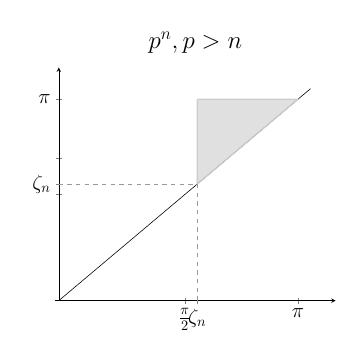
\begin{tikzpicture}[scale=0.52]
	\begin{axis} [
		title = {\LARGE $\Hbarc{p}{\VS^n}, p>n$},
		ticklabel style = {font=\Large},
		axis y line=middle,
		axis x line=middle,
		ytick={0.5,0.55,0.67,0.95},
		yticklabels={,$\zeta_n$,,$\pi$},
		xtick={0.5,0.55,0.95},
		xticklabels={$\frac{\pi}{2}$,$\zeta_n$, $\pi$},
		xmin=-0.015, xmax=1.1,
		ymin=0, ymax=1.1,]
		\addplot [mark=none] coordinates {(0,0) (1,1)};
		\addplot [thick,color=black!20!white,fill=black!30!white,
		fill opacity=0.4]coordinates {
			(0.55,0.95)
			(0.55,0.55)
			(0.95,0.95)
			(0.55,0.95)};
		\addplot [black!40!white,mark=none,dashed, thin] coordinates {(0,0.55) (0.55,0.55)};
		\addplot [black!40!white,mark=none,dashed, thin] coordinates {(0.55,0) (0.55,0.55)};
		%\node[mark=none] at (axis cs:0.68,0.21){$\Hbarc{p}{\VS^n}, p\geq 3$};
	\end{axis}
\end{tikzpicture}

\begin{tikzpicture}[scale=0.52]
	\begin{axis} [
		title = {\LARGE $\Hbarc{p}{X},1\leq p\leq n$},
		ticklabel style = {font=\Large},
		axis y line=middle,
		axis x line=middle,
		ytick={0.5,0.67,0.95},
		yticklabels={$\frac{\pi}{2}$,$\frac{2\pi}{3}$,$\pi$},
		xtick={0.5,0.67,0.95},
		xticklabels={$\frac{\pi}{2}$,$\frac{2\pi}{3}$,$\pi$},
		xmin=-0.015, xmax=1.1,
		ymin=0, ymax=1.1,]
		\addplot [mark=none] coordinates {(0,0) (1,1)};
		\addplot [thick,color=black!20!white,fill=black!30!white,
		fill opacity=0.4]coordinates {
			(0.67,0.95)
			(0.67,0.67)
			(0.95,0.95)
			(0.67,0.95)};
		\addplot [black!40!white,mark=none,dashed, thin] coordinates {(0,0.67) (0.67,0.67)};
		%\addplot [black!40!white,mark=none,dashed, thin] coordinates {(0,0.72) (0.72,0.72)};
		\addplot [black!40!white,mark=none,dashed, thin] coordinates {(0.67,0) (0.67,0.67)};
		\addplot[barccolor,mark=*] (0, 0.67) circle (2pt) node[above right,barccolor]{};%{\Large\textsf{1}};
		%\node[mark=none] at (axis cs:0.68,0.21){$\Hbarc{1}{X}$};
	\end{axis}
\end{tikzpicture}
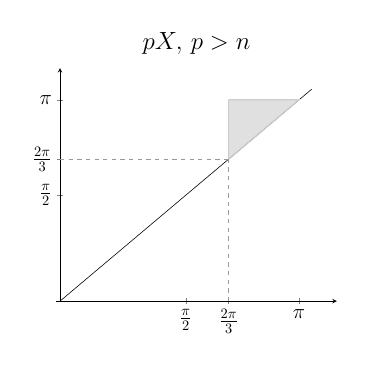
\begin{tikzpicture}[scale=0.52]
	\begin{axis} [
		title={\LARGE $\Hbarc{p}{X},\, p>n$},
		ticklabel style = {font=\Large},
		axis y line=middle,
		axis x line=middle,
		ytick={0.5,0.67,0.95},
		yticklabels={$\frac{\pi}{2}$,$\frac{2\pi}{3}$,$\pi$},
		xtick={0.5,0.67,0.95},
		xticklabels={$\frac{\pi}{2}$,$\frac{2\pi}{3}$,$\pi$},
		xmin=-0.015, xmax=1.1,
		ymin=0, ymax=1.1,]
		\addplot [mark=none] coordinates {(0,0) (1,1)};
		\addplot [thick,color=black!20!white,fill=black!30!white,
		fill opacity=0.4]coordinates {
			(0.67,0.95)
			(0.67,0.67)
			(0.95,0.95)
			(0.67,0.95)};
		\addplot [black!40!white,mark=none,dashed, thin] coordinates {(0,0.67) (0.67,0.67)};
		\addplot [black!40!white,mark=none,dashed, thin] coordinates {(0.67,0) (0.67,0.67)};
		% \addplot[barccolor,mark=*] (0, 0.67) circle (2pt) node[above right,barccolor]{\Large\textsf{1}};
		% \node[mark=none] at (axis cs:0.68,0.21){$\Hbarc{p}{X},\, p\geq 2$};
	\end{axis}
\end{tikzpicture}
% 	\caption{Barcodes of $\VS$ and barcodes of $X$.}
% 	\label{fig:VS_X}
% \end{figure}

% \begin{figure}[ht]
% 	\centering
% 	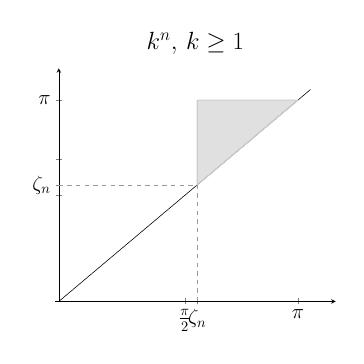
\begin{tikzpicture}[scale=0.52]
	\begin{axis} [
		title={\LARGE $\sqbarc{k}{\VS^n},\, k\geq 1$},
		ticklabel style = {font=\Large},
		axis y line=middle,
		axis x line=middle,
		ytick={0.5,0.55,0.67,0.95},
		yticklabels={,$\zeta_n$,,$\pi$},
		xtick={0.5,0.55,0.95},
		xticklabels={$\frac{\pi}{2}$,$\zeta_n$, $\pi$},
		xmin=-0.015, xmax=1.1,
		ymin=0, ymax=1.1,]
		\addplot [mark=none] coordinates {(0,0) (1,1)};
		\addplot [thick,color=black!20!white,fill=black!30!white,
		fill opacity=0.4]coordinates {
			(0.55,0.95)
			(0.55,0.55)
			(0.95,0.95)
			(0.55,0.95)};
		\addplot [black!40!white,mark=none,dashed, thin] coordinates {(0,0.55) (0.55,0.55)};
		\addplot [black!40!white,mark=none,dashed, thin] coordinates {(0.55,0) (0.55,0.55)};
		%\node[mark=none] at (axis cs:0.68,0.21){$\sqbarc{k}{\VS^n},\, k\geq 1$};
	\end{axis}
\end{tikzpicture}

\begin{tikzpicture}[scale=0.52]
	\begin{axis} [
		title = {\LARGE $\sqbarc{k}{\rp^n},\,1\leq k\leq n-1$},
		ticklabel style = {font=\Large},
		axis y line=middle,
		axis x line=middle,
		ytick={0.5,0.67,0.95},
		yticklabels={$\frac{\pi}{2}$,$\frac{2\pi}{3}$,$\pi$},
		xtick={0.5,0.67,0.95},
		xticklabels={$\frac{\pi}{2}$,$\frac{2\pi}{3}$,$\pi$},
		xmin=-0.015, xmax=1.1,
		ymin=0, ymax=1.1,]
		\addplot [mark=none] coordinates {(0,0) (1,1)};
		\addplot [thick,color=black!20!white,fill=black!30!white,
		fill opacity=0.4]coordinates {
			(0.67,0.95)
			(0.67,0.67)
			(0.95,0.95)
			(0.67,0.95)};
		\addplot [black!40!white,mark=none,dashed, thin] coordinates {(0,0.67) (0.67,0.67)};
		%\addplot [black!40!white,mark=none,dashed, thin] coordinates {(0,0.72) (0.72,0.72)};
		\addplot [black!40!white,mark=none,dashed, thin] coordinates {(0.67,0) (0.67,0.67)};
		\addplot[barccolor,mark=*] (0, 0.67) circle (2pt) node[above right,barccolor]{\Large$\geq$\textsf{1}};
	\end{axis}
\end{tikzpicture}
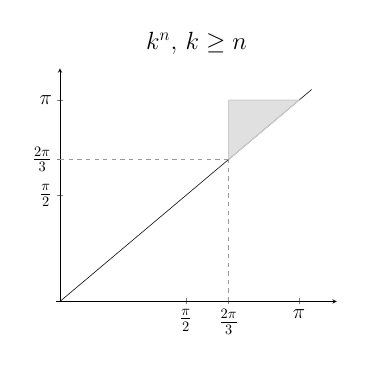
\begin{tikzpicture}[scale=0.52]
	\begin{axis} [
		title={\LARGE $\sqbarc{k}{\rp^n},\,k\geq n$},
		ticklabel style = {font=\Large},
		axis y line=middle,
		axis x line=middle,
		ytick={0.5,0.67,0.95},
		yticklabels={$\frac{\pi}{2}$,$\frac{2\pi}{3}$,$\pi$},
		xtick={0.5,0.67,0.95},
		xticklabels={$\frac{\pi}{2}$,$\frac{2\pi}{3}$,$\pi$},
		xmin=-0.015, xmax=1.1,
		ymin=0, ymax=1.1,]
		\addplot [mark=none] coordinates {(0,0) (1,1)};
		\addplot [thick,color=black!20!white,fill=black!30!white,
		fill opacity=0.4]coordinates {
			(0.67,0.95)
			(0.67,0.67)
			(0.95,0.95)
			(0.67,0.95)};
		\addplot [black!40!white,mark=none,dashed, thin] coordinates {(0,0.67) (0.67,0.67)};
		\addplot [black!40!white,mark=none,dashed, thin] coordinates {(0.67,0) (0.67,0.67)};
	\end{axis}
\end{tikzpicture}
% 	\caption{Barcodes of $\bS^n$, for $n\geq 2$ and degrees $m\geq 2$.
% 		Here, $\zeta_n=\arccos(-\tfrac{1}{n+1})$.
% 		In each figure, the gray area represents the only region, apart from the blue dots, where points could potentially exist within the corresponding barcode.}
% 	\label{fig:Sq_VS_X}
% \end{figure}

\subsection{Upper bound on $\db$ between usual barcodes}

To obtain an upper bound on the bottleneck distance, it suffices to find one matching and compute the cost of it. 

For any degree $1\leq m\leq n$, consider the matching $m$ between $\Hbarc{m}{\VS}$ and $\Hbarc{m}{X}$ such that $(0,\zeta_m) \leftrightarrow (0, \beta_m)$ and all other bars unmatched. 
Then the cost of $m$ satisfies
\begin{align*}
    \cost(m) 
    = & \max\{|\zeta_m - \beta_m|, \tfrac{\pi - \zeta_n}{2}, \tfrac{\pi - \alpha}{2}\} \\
    = & \max\{|\zeta_m - \beta_m|, \tfrac{\pi - \zeta_n}{2}\} && \mbox{(because $\zeta_n \leq \alpha$)}.
\end{align*}

Therefore, 
\begin{equation}\label{eq:db_usual_upper_bound}
    \db(\Hbarc{m}{\VS^n}, \Hbarc{m}{X})
    \leq \cost(m) 
    \leq \max\{|\zeta_m - \beta_m|, \tfrac{\pi - \zeta_n}{2}\}.
\end{equation}

% For any degree $m > n$, consider the matching $m$ between $\Hbarc{m}{\VS}$ and $\Hbarc{m}{X}$ such that all bars are unmatched. Then the cost of $m$ satisfies:
% \[
%     \cost(m) 
%     = \max\{\tfrac{\pi - \zeta_n}{2}, \tfrac{\pi - \alpha}{2}\} 
%     = \tfrac{\pi - \zeta_n}{2}. 
% \]

\subsection{Lower bound on $\db$ between $\theta$-barcodes}

To obtain a lower bound on the bottleneck distance, it suffices to calculate the minimum cost of matching a certain bar. 

For $k\in $ and $m\in $ \ling{need to specify the domain for $k$ and $m$}, we calculate the minimum cost of matching the bar $(0,\gamma_m) \in \thetabarc{X}$. 
Let $Q$ be an arbitrary matching between $\thetabarc{\VS}$ and $\thetabarc{X}$.
If $(0,\gamma_m)$ is unmatched in $Q$, then $\cost(Q) \geq \tfrac{\gamma_m}{2}$. 
If $(0,\gamma_m)$ is matched to some bar $(a,b)$ in $\thetabarc{\VS}$, then 
\begin{align*}
    \cost(Q) 
    = & \|(0,\gamma_m) - (a,b)\|_\infty \\
    = & \max\{a, |\gamma_m - b|\} \\
    \geq & \max\{\zeta_n, |\gamma_m - b|\} && \mbox{(because $a\geq \alpha \geq \zeta_n$)}\\
    = & \zeta_n.
\end{align*}
Here, the last equality holds because 
\[
    \gamma_m, b \in (\zeta_n, \pi)
    \implies |\gamma_m - b| \leq \pi - \zeta_n \leq \zeta_n.
\]
Thus,
\[
    \cost(Q) 
    \geq \min\{\tfrac{\gamma_m}{2}, \zeta_n\} 
    = \tfrac{\gamma_m}{2} 
    \geq \tfrac{\zeta_n}{2} 
\]

Therefore, 
\begin{equation}\label{eq:db_theta_lower_bound}
    \db(\thetabarc{\VS^n}, \thetabarc{X})
    \geq \min_Q \cost(Q) 
    \geq \tfrac{\zeta_n}{2}.
\end{equation}

\subsection{Conclusion}

We prove the lemma below to conclude that the lower bound of the bottleneck distance $\db$ between the $\theta$-barcodes of the two space $\VS^n$ and $X$ (Equation (\ref{eq:db_theta_lower_bound}))  is larger than the upper bound of $\db$ between the standard barcodes of the two spaces (Equation (\ref{eq:db_usual_upper_bound})). 
Thus, the $\theta$-barcodes provide a better (lower-bound) approximation of the Gromov--Hausdorff distance than $\db$ between the standard barcodes.

\lemma Since $\beta_m\in [\alpha, \tfrac{\zeta_n}{2}+\zeta_m)$, we have 
\[
    \max\{|\zeta_m - \beta_m|, \tfrac{\pi - \zeta_n}{2}\}
    \leq \tfrac{\zeta_n}{2}.
\]

To prove the lemma, consider two cases. 
If $\beta_m \leq \zeta_m$, then because $\tfrac{\pi}{2} \leq \beta_m\leq \zeta_m \leq \tfrac{2\pi}{3}$ and $\zeta_n \leq \tfrac{2\pi}{3}$, we have
\[
    |\zeta_m - \beta_m| 
    = \zeta_m - \beta_m 
    < \tfrac{2\pi}{3} - \tfrac{\pi}{2} 
    = \tfrac{\pi}{6} 
    < \tfrac{\pi - \zeta_n}{2}.
\]
Thus, $\max\{|\zeta_m - \beta_m|, \tfrac{\pi - \zeta_n}{2}\} = \tfrac{\pi - \zeta_n}{2} \leq \tfrac{\zeta_n}{2}.$

If $\beta_m>\zeta_m$, then because $\beta_m <\tfrac{\zeta_n}{2}+\zeta_m$, we have
\[
    \max\{|\zeta_m - \beta_m|, \tfrac{\pi - \zeta_n}{2}\}
    < \max\{\tfrac{\zeta_n}{2}, \tfrac{\pi - \zeta_n}{2}\}
    = \tfrac{\zeta_n}{2} .
\]

\example For the real-projection plane $\rp^n$, the first critical value of $\VR(\rp^n)$ and the $m$-the homology of $\VR(X)$ are both $\tfrac{2\pi}{3}$. %, i.e. $\alpha = \beta_m = \tfrac{2\pi}{3}.$ 
It is clear that $\alpha= \tfrac{2\pi}{3}$ lies in $(\zeta_n, \pi)$ and $\beta_m= \tfrac{2\pi}{3} < \tfrac{\zeta_n}{2}+\zeta_m.$

\ling{Mention $\theta$ is Steenrod here.}


\subsection{First critical value of $\opH_m(\VR(\rp^n))$}

In this section, we show that for any degree $1 \leq m \leq n$, the first critical value of the $m$-th homology of the Vietoris-Rips filtration of $\rp^n$ is $\tfrac{2\pi}{3}.$

We fix some $n\geq 2.$

\subsubsection{}

\ling{We need to be careful with the citation here: (1) cite \cite{adams2022metric} for the original definition; (2) cite Liam Barham for the fixed definition. 
We should ask Liam Barham for permission to cite his unpublished work.}

Let $G$ be a group acting properly and by isometries on a metric space $X$.
Let $t_0>0$. The action of a group $G$ on $X$ is an \defn{$t_0^*$-diameter action} if for any non-negative integer $k$, $\diam_{X_G}\{[x_0],\dots,[x_k]\}<t_0$ implies that there exist unique choice of $g_i$'s for $1\leq i\leq k$ such that $\diam_{X}\{x_0,g_1x_1,\dots,g_kx_k\}<t_0$. 

Assume the action of $G$ on $X$ is a $t_0^*$-diameter action for some $t_0> 0$.
In \cite[Proposition 3.5]{adams2022metric}, the authors constructed a homomeorphism from $\VR_t^m(X_G)$ to $\VR_t^m(X)/G$ for all $t \leq t_0$.
We review their constructions below. 

Define the map $h$ to be
\[
h \colon \VR_t^m(X) \to \VR_t^m(X_G) 
\text{ with }
\sum_{i=1}^k \lambda_i x_i \mapsto \sum_{i=1}^k \lambda_i [x_i],
\]
Because $G$ acts isometrically, $h$ is well-defined.
Because two points in the same orbit of the $G$ action always have the same image under $h$, it induces a map $h/G \colon \VR_t^m(X)/G \to \VR_t^m(X_G)$.
Moreover, $h/G$ is an isomorphism, following from the fact that the action of $G$ on $X$ is an $r^*$-diameter action; see \cite[Proposition 3.5]{adams2022metric} for further details.

Assuming that the action of $G$ on $X$ is a $t_0^*$-diameter action, for any $0<t<t_0$, we can consider the inverse of $h/G$ and we denote it as
\[
h \colon \VR_t^m(X_G) \to \VR_t^m(X)/G
\text{ with }
\sum_{i=1}^k \lambda_i [x_i] \mapsto [\sum_{i=1}^k \lambda_i x_i].
\]


\subsubsection{}

Let $\bS^n$ the sphere of radius $2$ and let $G=\Z/2\Z$ act on $\bS^n$ by identifying the antipodal points.
It follows from \cite[Corollary]{adams2022metric} that the action of $G$ on $\bS^n$ is a $t^*$-diameter action for any $t<\tfrac{2\pi}{3}$.

For any $t<\pi$, let $\tilde{f}^n$ be the composition
\[
    \tilde{f}^n \colon \VR_t^m(\bS^n) \to \R^{n+1} \setminus \set{0} \xra{\pi^n} \bS^n,
\]
where the first map sends a formal linear sum $\sum_{i=1}^k \lambda_i x_i$ in the Vietoris--Rips thickening $\VR_t^m(\bS^n)$ to the point $\sum_{i=1}^k \lambda_i x_i \in \bbR^{n+1}$ where $x_i \in \bS^n$ and $\lambda_i \in [0,1]$ satisfying $\sum_i\lambda_i=1$, and the second map $\pi^n$ is the radial projection map.

By \cite[Proposition 5.3]{adamaszek2018metric}, the map $\tilde{f}^n$ is a homotopy equivalence for all $0<t<\zeta_n=\arccos{(-\tfrac{1}{n+1})}$.
% When $n=1$, this is $\tfrac{4\pi}{3}.$

\ling{To Anibal: please check that $\tilde{f}^n/G$ is well-defined for lens spaces and if it is a homotopy equivalence. }

Because $\tilde{f}^n$ preserves group action, i.e. $\tilde{f}^n(x) = \tilde{f}^n(gx)$ for any $x\in \bS^n$ and $g\in G$, we have the homotopy equivalence for $0<t<\zeta_n$, %\anibal{Maybe use superscripts for these maps and the $\rho$ too?}
\[
\tilde{f}^n/G \colon 
\VR_t^m(\bS^n)/G \, 
\to \bS^n_G.
%\cong \rp^n.
\]
By composing $h^n$ with $\tilde{f}^n/G$, we obtain a map 
\[
\rho^n = h^n \circ \tilde{f}^n/G 
\colon \VR_t^m(\bS^n_G) \to \bS^n_G
\]

\subsubsection{} 

For $0<t\leq s \leq s'$, we consider the following diagram of topological spaces:
\begin{equation}\label{d:fundamental_bars_diagram}
    \begin{tikzcd}
        \bS^{n-1}_G
        \ar[d, hook,"{\iota}" left]
        &
        \VR_t(\bS^{n-1}_G)
        \ar[d, hook,"\iota_t"]
        \ar[l, "\rho^{n-1}" above, "\simeq" below]
        \ar[r, hook, "v^{n-1}"]
        &
        \VR_{s}(\bS^{n-1}_G)
        \ar[d, hook]
        \\
        \bS^{n}_G
        &
        \VR_t(\bS^{n}_G)
        \ar[l, "\rho^n" below, "\simeq" above]
        \ar[r, hook, "v^{n}"]
        &
        \VR_{s'}(\bS^{n}_G).
    \end{tikzcd}
\end{equation}
Here, the horizontal inclusions $v^{n-1}$ and $v^n$ are induced by the Vietoris--Rips filtration, whereas the vertical maps are induced by the equatorial inclusion of real projective spaces $\iota \colon \bS^{n-1}_G \hookrightarrow \bS^{n}_G$.

We claim that diagram \eqref{d:fundamental_bars_diagram} commutes. 
The commutativity of the right-hand-side square is straightforward.
For the left-hand-side square, we need to verify that $\iota \circ \rho^{n-1}=\rho^{n} \circ \iota_t$.
\ling{notation for maps below need to be fixed at the end.}
Indeed, for any $y = \sum_{i=1}^k \lambda_i [x_i] \in \VR_t(\bS^{n-1}_G)$, we have
\begin{center}
    $(\iota \circ \rho^{n-1})(y)
    =\iota(f^{n-1}/\sim([\sum_i \lambda_i x_i]))
    =\iota([f^{n-1}(\sum_i \lambda_i x_i)])
    =[\pi^{n-1}(\sum_i \lambda_i x_i)]
    $
\end{center}
as an element in $\bS^n_G$, and
\begin{center}
    $(\rho^{n} \circ \iota_t)(y) = \rho^{n}(y) = f^{n}/\sim([\sum_i \lambda_i x_i]) = [f^{n}(\sum_{i=1}^k \lambda_i x_i)] = [\pi^{n}(\sum_{i=1}^k \lambda_i x_i)]
    $
\end{center}
Because $\pi^{n}$ restricted to $\bS^{n-1}_G$ is equal to $\pi^{n-1}$, we conclude that $(\iota \circ \rho^{n-1})(y) = (\rho^n \circ \iota_t)(y)$ for any $y$.
Thus, the claim holds.

\subsubsection{}

\lemma For integers $1 \leq m \leq n$,
\[
\left(0, \tfrac{2\pi}{3}\right) \in \Hbarc{m}{\bS^n_G}.
\]

\ling{We need the first critical value of the $m$-th homology of $\bS^n_G$ for all $1\leq m\leq n-1$ and all $n.$}

\begin{proof}
	We will use an induction argument on $n$.
	When $n = 1$, \cref{ss:filling_radius} implies that
 \ling{here we need the filling radius of $\bS^1/G$}
	\[
	(0, 2\fillrad{\rp^1}) = \left(0, \tfrac{2\pi}{3}\right) \in \Hbarc{1}{\rp^1}.
	\]
	Assume the statement holds for $\bS^{n-1}_G$.
	% That is, for any $1 \leq m \leq n-1$,
	% \[
	% \left(0, \tfrac{2\pi}{3}\right) \in \Hbarc{m}{\bS^{n-1}_G}.
	% \]

    For the case when $1\leq m\leq n-1$, applying the $m$-th homology functor (over $\Ftwo$ \ling{replace with a suitable field}) to diagram \eqref{d:fundamental_bars_diagram}, we obtain the following commutative diagram of vector spaces:
    \ling{For the first $\frac{2\pi}{3}$, we want to replace it with a value such that $\rH_m(v^{n-1})$ is zero. 
    The first critical value may not be enough (unless the homology is always at most dimension one): changing type is different from being zero.}
    \[
    \begin{tikzcd}
        \rH_m(\bS^{n-1}_G)
        \ar[d, "\cong" left]
        &
        \rH_m(\VR_t(\bS^{n-1}_G))
        \ar[d, "\rH_m(\iota_t)" left, "\cong" right, myred]
        \ar[l, "\cong" above]
        \ar[rr, "\rH_m(v^{n-1})=0", myred]
        &
        &
        \rH_m(\VR_{\tfrac{2\pi}{3}+\epsilon}(\bS^{n-1}_G))
        \ar[d]
        \\
        \rH_m(\bS^{n}_G)
        &
        \rH_m(\VR_t(\bS^{n}_G))
        \ar[l, "\cong"]
        \ar[rr, "\rH_m(v^n)" , myred]
        &
        &
        \rH_m(\VR_{\tfrac{2\pi}{3}+\epsilon}(\bS^{n}_G)).
    \end{tikzcd}
    \]
    Here, $\rH_m(g)$ for some map $g$ between topological spaces denotes the induced map of $g$ on the $m$-th homology. 

    Commutativity of the left-hand-side square implies that $\rH_m(\iota_t)$ is an isomorphism.
    By induction assumption, $(0, \tfrac{2\pi}{3})\in\Hbarc{m}{\bS^{n-1}_G}$, which implies that $\rH_m(v^{n-1})$ is the zero map.
    Then, using the right-hand-side square's commutativity, we deduce $\rH_m(v^n) \circ \rH_m(\iota_t)=0$.
    Since $\rH_m(\iota_t)$ is an isomorphism, we conclude that $\rH_m(v^n)=0$.
    This holds for any $\epsilon>0$, so we can conclude $(0, \tfrac{2\pi}{3})\in\Hbarc{m}{\bS^{n}_G}$.
	
	For the case when $m=n$, we can apply the lemma in \textsection \ref{ss:filling_radius} to obtain 
    \[
    (0,2\fillrad{\bS^n_G}) = (0, \tfrac{2\pi}{3}) \in \Hbarc{n}{\bS^n_G}.
    \]
        
	Therefore, $(0, \tfrac{2\pi}{3}) \in \Hbarc{m}{\bS^n_G}$ is established for all $1\leq m\leq n.$
\end{proof}

We will refer to the bar in this lemma as the \defn{fundamental bar} of $\bS^n_G$.
